\chapter{Estrategia de resolución}

En este capitulo se explica el proceso llevado a cabo para desarrollar la solucion. Se presenta el modelado basico del problema que consiste en un mapa de la zona con todos los datos necesarios para realizar la simulacion y el algoritmo genetico utilizado con su estructura, parámetros y configuración. 

Se detalla la biblioteca utilizada para el desarrollo del algoritmo y la arquitectura desarrollada.



\section{Modelado del problema }

Para solucionar el problema se usaran simulaciones de la realidad, por tanto es importante contar con un modelo detallado y fidedigno.
A continuacion se detallan los puntos destacados del modelo.




\subsection{Representaciones}

\subsubsection{Red de calles}
La red de calles se representa como un grafo dirigido en un archivo xml con extensión .net.xml . Allí se especifican los nodos, y vértices así como sus atributos. También se representan los semáforos. Esto  se genera utilizando una herramienta  para convertir un mapa al formato que SUMO utiliza.

\subsubsection{Representación tráfico}
En este caso también se utiliza un archivo xml donde se definen las rutas y los recorridos. Un recorrido representa el movimiento de un vehículo de un punto inicial hacia un punto final (El recorrido se hacen en tiempo de ejecución utilizando el camino más corto basado en el tráfico). 


\subsubsection{Representación del tiempo}
El tiempo se representa como una serie de pasos discretos, cada uno durando un segundo. Este valor se puede modificar aunque es recomendado dejarlo así para que sea consistente.


\subsubsection{Tipos de vehículos}
Se pueden crear diferentes tipos de vehículos especificando propiedades como largo, velocidad máxima,  aceleración, color, etc. También cuenta con vehículos por defecto como buses, camiones o automóviles.

\subsection{Configuración de la simulación}

En esta sección se realiza un resumen sobre los pasos realizados para tener los elementos necesarios para realizar la simulación.

\subsubsection{Diseño del mapa}


El mapa base de la zona proviene de Open Street Map \citep{OSM}, luego se cotejó su exactitud con Google Maps y Bing Maps.

\begin{figure}[H]
	\centering
	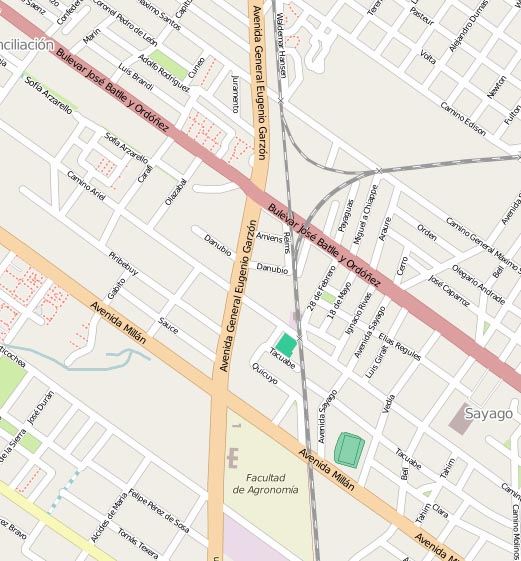
\includegraphics[width=0.7\linewidth]{Figures/osm_garzon}
	\caption{Tramo del mapa de Garzon de OSM}
	\label{fig:osm_garzon}
\end{figure}


Se utilizó la herramienta netconvert para convertirlo al formato que SUMO acepta. 
Para esto se realizaron varios ajustes editando los archivos xml para corregir errores en las calles, cruces y conexiones para que fuese fiel a la realidad y mantuviera la compatibilidad con SUMO.


\begin{figure}[H]
	\centering
	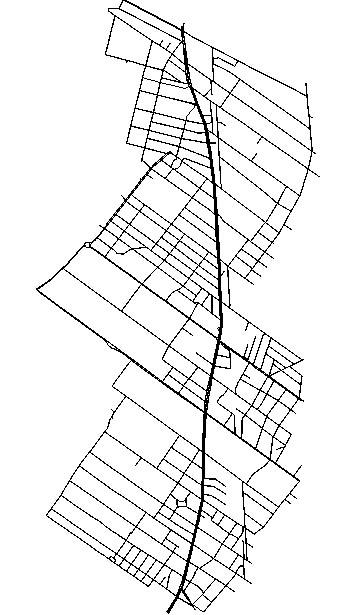
\includegraphics[width=0.5\linewidth]{Figures/mapa_sumo}
	\caption{Mapa cargado en SUMO luego del modelado y procesamiento}
	\label{fig:mapa_sumo}
\end{figure}



\section{Trabajo de campo}
Al no contar con datos públicos sobre la densidad de trafico en la zona, realizamos un revelamiento in-situ con las siguientes características.

Se seleccionaron cinco cruces que presentan diferentes características para poder modelar variantes en la cantidad de vehiculos circulantes.
Estos son: Camino Ariel, Battle y Ordoñez, Plaza Videla, Camino Colman y Aparicio Saravia.

Se siguen las recomendaciones de los textos consultados al respecto \citep{ConteoTrafico}. Se eligió el día miércoles, que estuviera soleado y entre las 15 y 17 horas para no tener los sesgos que se producen los fines de semana o días de lluvia.
Se realizaron filmaciones de entre 15 y 30 minutos en los cruces y luego se analizaron los vídeos para realizar el conteo manual con la posibilidad de enlentecer el vídeo para mayor facilidad. Luego se completa una planilla electrónica donde se tiene la información de vehículos que recorren Garzón, la calle que cruza y los que doblan. También discriminamos entre vehículos y ómnibus que recorren Garzón.

\begin{figure}[H]
	\centering
	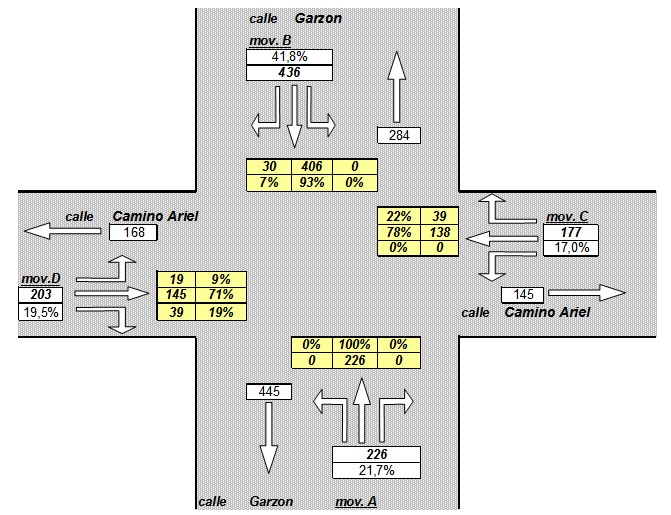
\includegraphics[width=0.7\linewidth]{Figures/conteo_hoja}
	\caption{Ejemplo de planilla electrónica para el conteo manual en Camino Ariel}
	\label{fig:conteo_hoja}
\end{figure}

(TABLA CON RESULTADOS DE TRAFICO)

Además se realizaron recorridas de punta a punta del corredor a una velocidad constante para verificar los tiempos obtenidos en la simulación para este recorrido.

Para obtener la configuración de los semáforos se realizo un recorrido en bicicleta por el corredor cronometrando la duración del tiempo en cada esquina de cada semáforo. Tanto de ida como de vuelta para corroborar que fueran correctos. Estos tiempos fueron verificados por los vídeos obtenidos.


\newpage
\subsubsection{Creación del modelo del tráfico}
Esta es la representación de la circulación de vehículos, aquí exponemos algunos de los más populares. 

Aleatorios: Genera diferentes recorridos que seguirán los vehículos aleatoriamente

JTR (junction turning ratio) : basados en probabilidades en los cruces  es decir cuando un vehículo llega a un cruce tiene cierta probabilidad de seguir o doblar.

Basado en áreas:  Se especifican áreas como un conjunto de calles y se realizan recorridos entre ellas.


Basado en Actividad: Se especifica la cantidad de casas, vehículos y población en un determinado lugar y el modelo genera la densidad de tráfico que se producirá basado en los tipos de actividades que se realizan comúnmente como ir al trabajo, hacer las compras, ir a la escuela,  etc

Definido por el usuario: que permiten determinar la ruta de los vehículos con mayor detalle.



Con los datos relevados se creo un modelo vehicular de la ciudad [poner el mapa] que brinda una aproximación sobre la densidad de tráfico y la velocidad promedio de circulación.

Se utilizó el programa Traffic Modeler \citep{TrafficModeler} con lo que se logra generar modelos de tráfico complejo de manera visual. Se optó por un modelo de movilidad entre áreas lo que permite una buena granularidad al especificar la densidad de tráfico.


\begin{figure}[H]
	\centering
	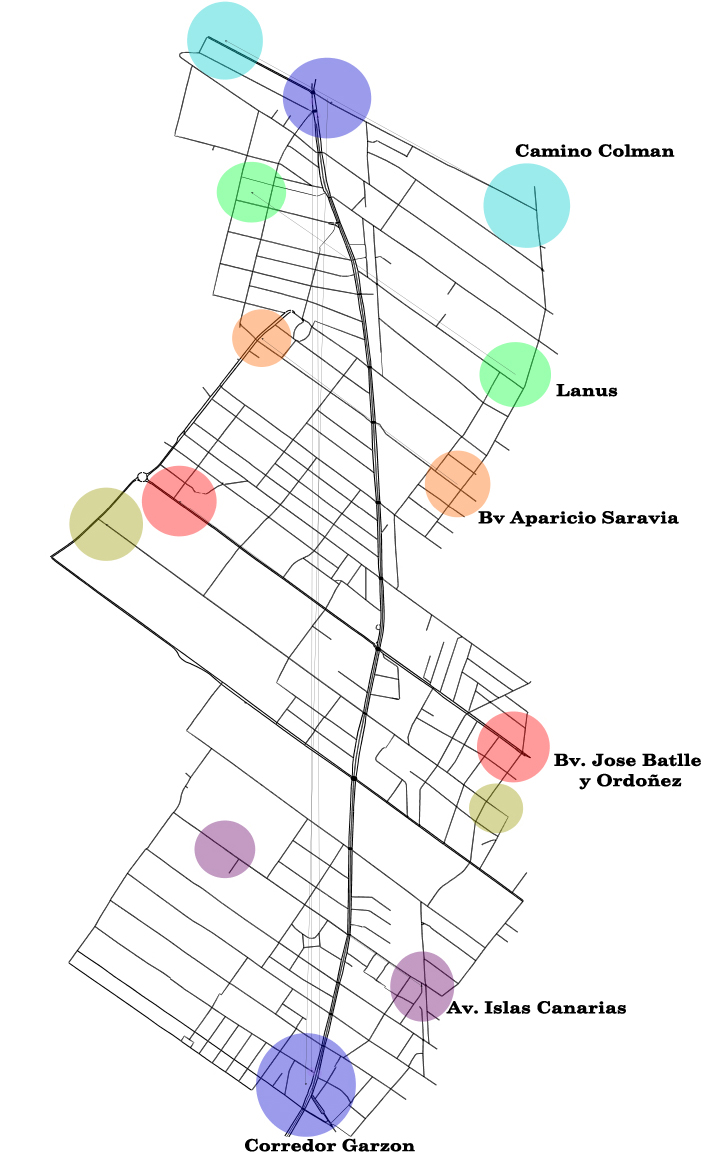
\includegraphics[width=0.4\linewidth]{Figures/areaflow1}
	\caption{Mapa del TrafficModeler con las áreas de tráfico. Círculos del mismo color indican tráfico especificado entre esas áreas}
	\label{fig:areaflow1}
\end{figure}


Actualmente no se cuenta con información publica relativa a la configuración de los semáforos en la ciudad, aunque cabe destacar que en el futuro se prevé crear un sistema centralizado de sincronización de semáforos. \citep{OBS01} 
En este caso se agregó la información sobre la configuración de los semáforos de los datos relevados.

Se manejaron dos tipos de vehículos autos y ómnibus cada uno con características distintas tanto de tamaño, aceleración y velocidad máxima.

Se agregaron las frecuencias y los distintos recorridos de los ómnibus obtenidos de datos públicos de la Intendencia Municpal de Montevideo \citep{IMM}
Estos incluyen las lineas urbanas  'G', '409' ,'2', 'd5'  y  '148' . 

Las líneas de ómnibus suburbanas realizan  un mismo  trayecto y las generalizamos con el nombre 'A' las cuales no van a ser tomadas en cuenta en la optimización del algoritmo pero si aparecerán en la simulación.

La ubicación y lineas de cada parada se obtuvo de \citep{sigMontevideo}, existen 14 paradas para lineas urbanas por el corredor para el recorrido de ida y las mismas para la vuelta.
Para los recorridos se hicieron  variantes  en  los  viajes  dentro  de  una  misma línea para simular el hecho de que no siempre se para en las mismas paradas.

También se tuvo en cuenta para la simulación el tiempo que demora un ómnibus al detenerse en una parada, y que hay algunas donde por la cantidad de gente se demora mas. Estos datos fueron obtenidos en el lugar considerando tiempos de entre 15 a 35 segundos.

Para establecer la velocidad media de los ómnibus se realizo un estudio basado en datos de GPS proporcionados por la IMM luego de reuniones con Ingenieria de Transito.
Estos datos cuentan con la posicion GPS, la velocidad instantanea y la referencia al omnibus para un conjunto de lineas seleccionadas tomadas en un periodo de una semana. Luego de procesar los datos se obtuvo una velocidad media de 14.5 km/h lo que permite ajustar mejor el modelo. 



\begin{figure}[h]
	\centering
	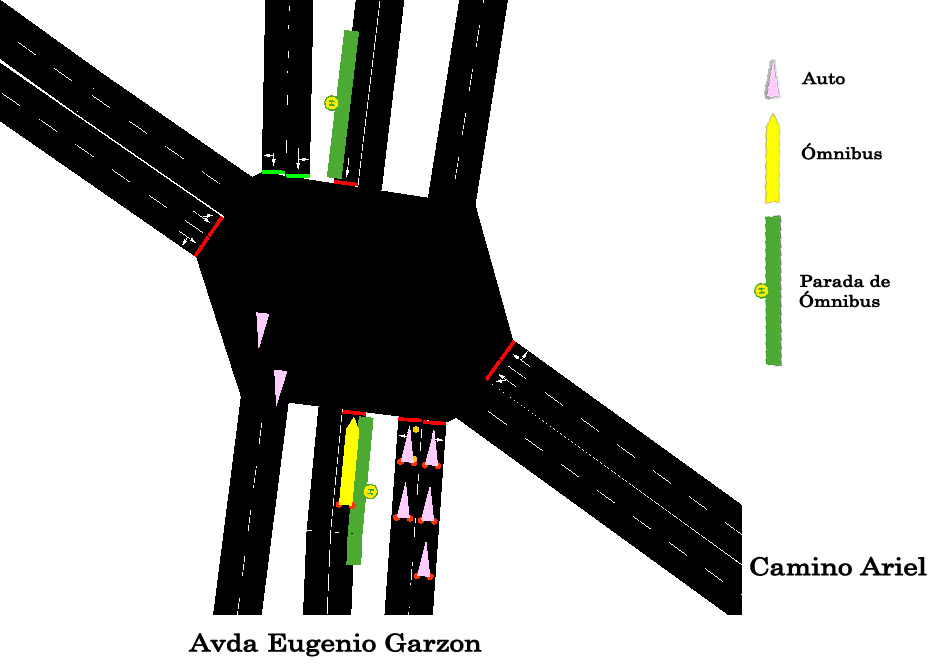
\includegraphics[width=0.7\linewidth]{Figures/sim1}
	\caption{Simulacion de tráfico en SUMO en el cruce entre Bulevar Battle y Ordoñez y el Corredor Garzon.}
	\label{fig:sim1}
\end{figure}


\section{Arquitectura de la solución}

En el siguiente diagrama muestra la arquitectura propuesta para el problema.

\begin{figure}[H]
\centering
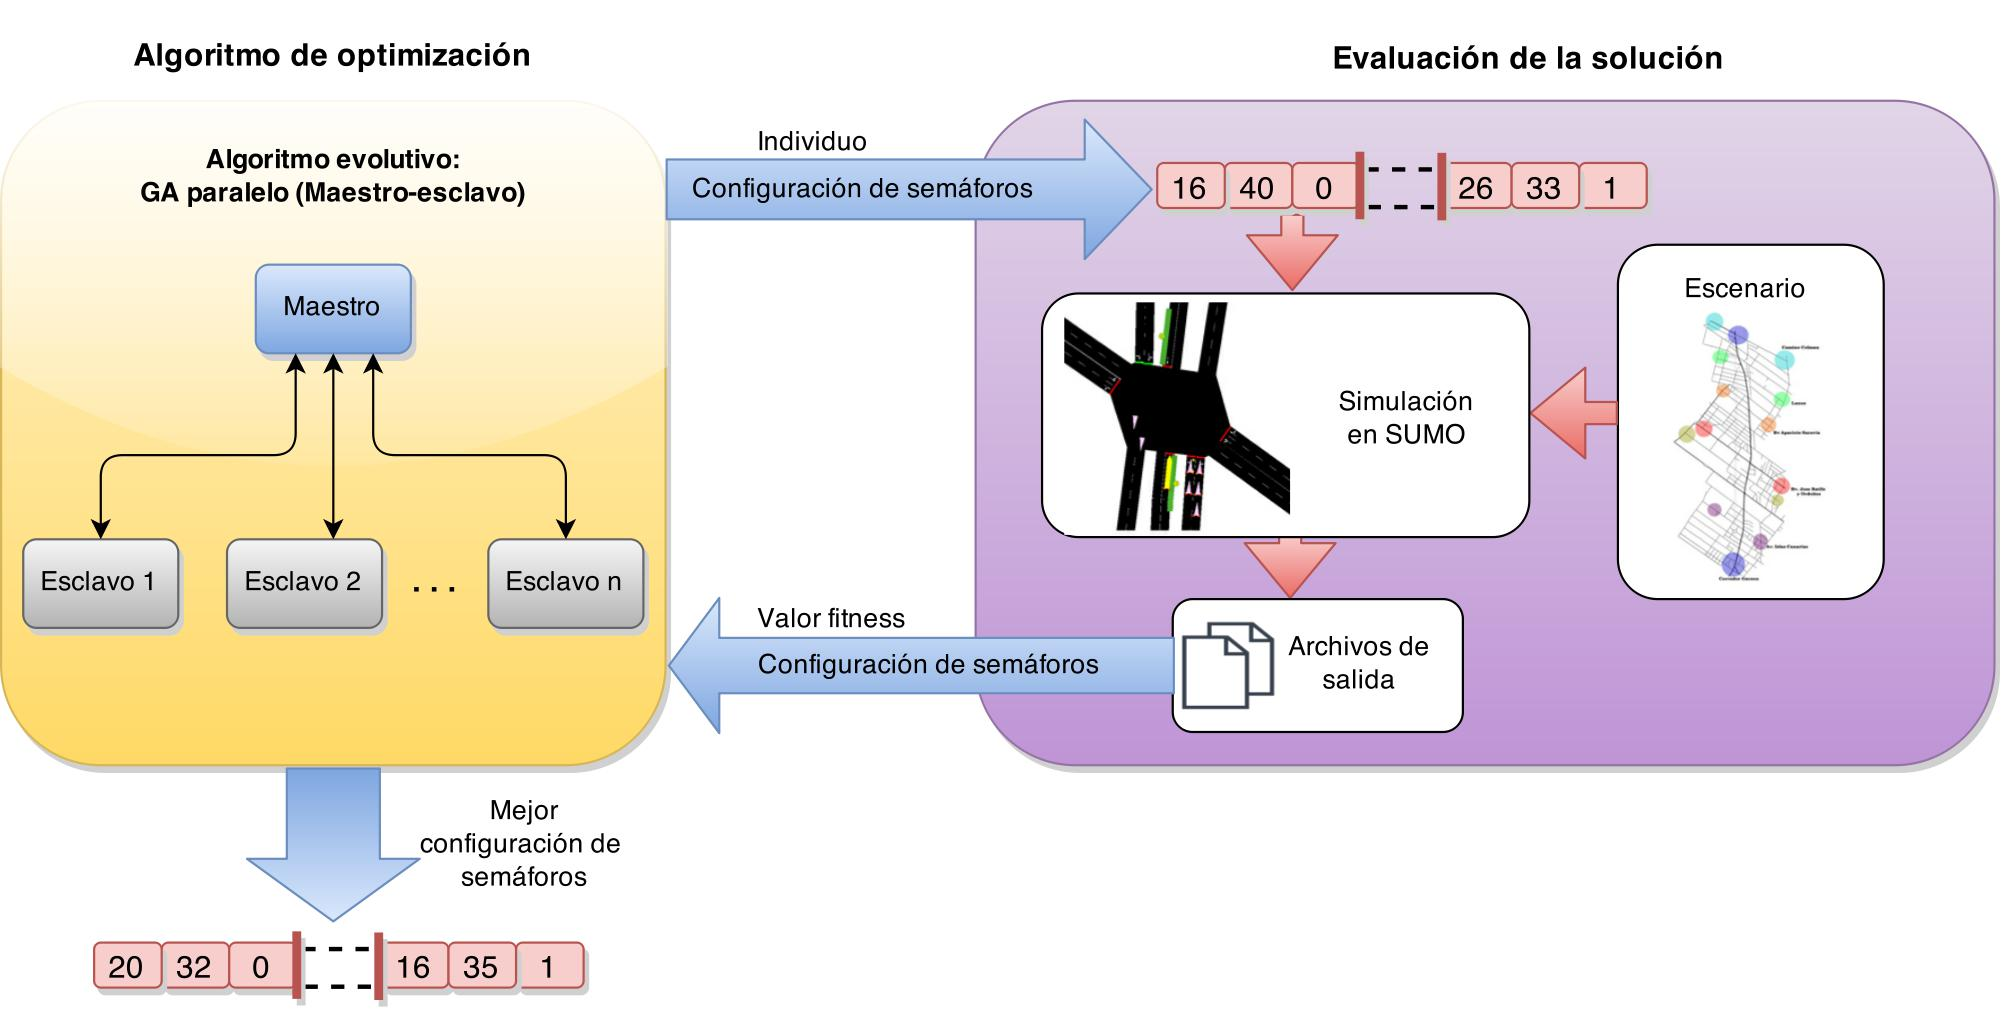
\includegraphics[width=0.7\linewidth]{Figures/arquitectura1}
\caption{Arquitectura del algoritmo}
\label{fig:arquitectura1}
\end{figure}


Malva se utiliza para la implementación del algoritmo, en cada evaluación de la función de fitness se realiza un llamado al simulador SUMO. 

El simulador genera archivos con información sobre la simulación que son usados por el algoritmo para determinar el fitness.

Luego los archivos son procesados por el algoritmo para extraer los datos útiles necesario para la función de fitness.







\section{Biblioteca Malva}

\citep{Malva} surge como una variante del proyecto \citep{Mallba}. Propone la actualización, mejora y desarrollarlo como un proyecto de código abierto colaborativo.  Su objetivo es proveer de varios esqueletos de  heurísticas de optimización que puedan ser utilizados y extendidos de manera fácil y eficiente.

Los esqueletos se basan en separar dos conceptos: El problema concreto que se quiere resolver y por otro lado el método utilizado para resolverlo. Por tanto un esqueleto se puede ver como una plantilla genérica que se instancia para resolver un problema particular, manteniendo todas las funcionalidades genéricas.

Utiliza el lenguaje c++ dado su alto nivel, modularidad y flexibilidad. Los esqueletos se ofrecen como un conjunto de clases requeridas que son las que el usuario deberá modificar para adaptarlo a su problema y las provistas. que incluyen todos los aspectos internos del esqueleto y on independientes del problema particular. Entre los algoritmos provistos se encuentra el de Algoritmos genéticos y \citep{CHC}.



\section{Herramientas}
Aquí se muestra información útil sobre las herramientas utilizadas.

\subsection{Open Street Map} 
Es un proyecto en donde una comunidad crea mapas libres y editables \citep{OSM}. Cuenta con cerca de 1.8 millones de usuarios  y  más de 20.000 que editaron algo en el ultimo mes \citep{OSMSTATS} por lo que es muy activa. Se utilizan datos de GPS móviles, fotografías satelitales y otras fuentes libres para crear los mapas y editarlos. 

\subsection{SUMO ( Simulation of Urban MObility)}

Es un simulador de tráfico gratis y abierto que nos permite modelar redes de calles, vehículos, transporte publico, ciudadanos y semáforos \citep{SUMO}. Sigue un modelo microscópico ya que realiza la simulación individual explicita de cada elemento. además incluye un conjunto de herramientas destinadas  a facilitar la generación de tráfico, construcción de mapas, etc. 


\subsection{Por que usar SUMO? }
otras alternativas? Revisar estado del arte?
Sumo es gratis
Nos permite utilizarlo sin interfaz gráfica por linea de comando lo que aumenta sensiblemente la velocidad ed ejecución, y  nos permite visualizar la interfaz gráfica una vez completada la optimización para ver exactamente como se comporta el sistema en la simulación.

Sumo presenta varias salidas con información interesante: \citep{SUMOOUT} 
La salida obtenemos el tiempo de simulación, la cantidad de emitidos y la cantidad de completados. Buscamos que sea > 80%
Permite la ejecución tanto por linea de comando como una interfaz gráfica para visualizar

\subsection{NetConvert}
Utilizado para la generación de la red a partir de un mapa. Por ejemplo podemos transformar un mapa de Open Street Map en archivo XML de red que SUMO reconoce. Este programa viene integrado con SUMO

\subsection{DUaRouter}
Genera recorridos de vehículos basado en dinámicas definidas por el usuario. Esta utilidad viene integrada con SUMO.

\subsection{Traffic Modeler}
Herramienta para la generación de tráfico de manera visual y luego transformarlo para que sea reconocido por SUMO. \citep{TrafficModeler}

\newpage

\section{Especificación del Algoritmo Genético utilizado}
Se utiliza el algoritmo genético proviso por la biblioteca  Malva  llamado NewGA al cual se le realizan algunas modificaciones para que se ejecute en paralelo.


Resumen de las características:
\begin{itemize}

\item Algoritmo paralelo: Utiliza el método maestro esclavo para que en cada iteración el maestro genere un hilo para cada ejecución  de la función fitness y luego espere a la terminación de todos los hilos para consolidar los datos. 
\item Función Multiobjetivo: Se intenta optimizar tanto la velocidad promedio de vehículos como de ómnibus teniendo cada uno un peso especifico.
\item Representación del cromosoma: Es un vector de números reales que representan los tiempos de los semáforos.
\item Cruzamiento y mutación: Se utiliza una variante del cruzamiento por un punto especifico para nuestro caso así como para la mutación.
\item Selección y reemplazo: Reemplaza padres por hijos, la selección de los padres se realiza por el método de torneo de 3 individuos, y la selección de hijos por el método de ruleta.

\end{itemize}

más adelante se realizara el ajuste paramétrico para determinar tanto el tiempo de simulación, criterio de parada y tasas de cruzamiento y mutación optimas para el algoritmo.

El siguiente esquema muestra el algoritmo utilizado. \citep{MalvaAlgGenetico}

 
\begin{algorithm}[H]
	\caption{Algoritmo Genético de Malva}
	\label{alg:algoritmo_genetico_malva}
	\begin{algorithmic} [1] 
		{
			\STATE \texttt{t} = 0
			\STATE {Inicializo( P(t))}
			\STATE {Evaluar estructuras en ( P(t))}			
			\WHILE {\text{No termine}}
			\STATE \texttt{t}++		
			\STATE {Seleccionar C(t) de P(t-1)}	
			\STATE {Recombinar estructuras en C(t) formando C'(t)}				
			\STATE {Mutar estructuras en C'(t) formando C''(t)}		
			\STATE {Evaluar estructuras en C''(t) generando un hilo de ejecucion por cada una}					
			\STATE {Consolidar valores de la evaluacion}								
			\STATE {Reemplazar P(t) de C''(t) y P(t-1)}								
			\ENDWHILE
		}
	\end{algorithmic}

\end{algorithm}




 

\subsection{Representación del cromosoma}

Se explican algunas definiciones necesarias para comprender la representación.

Cruce: Es el lugar de intersección de dos o más vías de circulación.
Fase: Es la configuración de las luces de los semáforos en un determinado cruce.

El  cromosoma  se  va  a  agrupar  lógicamente  en  cruces siendo el valor de cada gen el tiempo que demora una
fase de un cruce, además se agrega para cada cruce un número que representa en que fase comienza el semáforo. 
Por tanto el tamaño del cromosoma depende tanto de la cantidad de cruces como la cantidad de fases de cada uno.

En la representación se omiten las luces amarillas ya que no modifican los tiempos reales del paso de vehículos.
 
Es  importante que el algoritmo no genere soluciones inviables por lo que no debe modificar la combinación de luces de cada fase evitando combinaciones de luces erróneas. Por tanto tanto la modificación se realizara solo en el valor que indica el comienzo de fase y en los tiempos relacionados.

\begin{figure}[h]
\centering
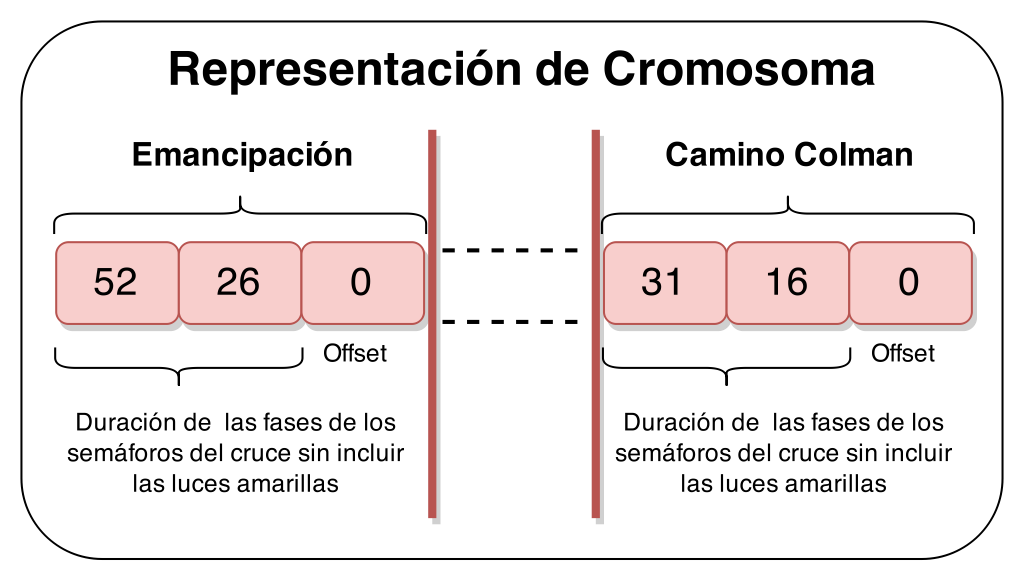
\includegraphics[width=0.7\linewidth]{Figures/cromosoma1}
\caption{Cromosoma de 2 cruces}
\label{fig:cromosoma1}
\end{figure}

En la siguiente figura vemos la representación de los archivos de simulación que nos provee SUMO para el cromosoma anterior, donde vemos como se representan las fases por ejemplo el texto “GGGGrrGGGGrr” demora 52 segundos. “G” es Verde, “r” es Rojo e “y” es Amarillo. El offset indica el inicio de la fase.

\begin{figure}[h]
\centering
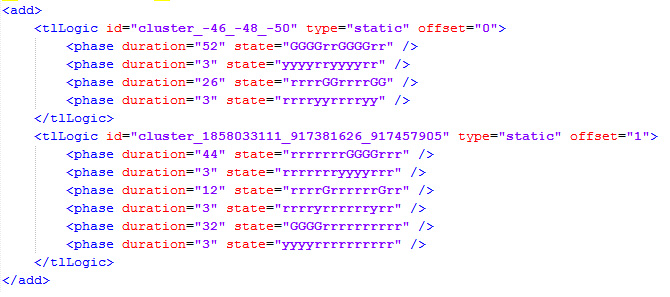
\includegraphics[width=\linewidth]{Figures/rep_sumo}
\caption{Representación de Sumo}
\label{fig:rep_sumo}
\end{figure}


\subsection{Inicialización}

Para la inicialización de la población se toma como referencia
la configuración obtenida con los datos in-situ, luego para cada
cruce se hacen variar las duraciones de las fases de manera aleatoria entre un rango de  5 a 60  segundos  (valores configurables)
además la fase inicial se elige aleatoriamente entre la cantidad de fases del cruce (se cuentan las luces amarillas).

\subsection{Función fitness}
La evaluación de un individuo se realiza generando un archivo con la configuración de los semáforos en base a su cromosoma y ejecutando el simulador SUMO utilizando esta configuración para luego obtener los tiempos necesarios para calcular el fitness.

Se empleara una funcion multiobjetivo usando combinacion lineal de la velocidad de los omnibus y del resto de los vehiculos, ya que es un metodo sencillo y adecuado cuando son menos de tres objetivos. El fitness se calcula como una suma ponderada, con los pesos fijados a priori.

        \begin{equation}
        \label{eq:funcion_fitness_generica}
		F(x) = \sum_{i=1}^{n}{w_i}{f_i}(x)
        \end{equation}

En nuestro caso tenemos como objetivo la velocidad promedio de los ómnibus (vpb) y la velocidad promedio del resto de los vehículos (vpv).

Esta es la formula de fitness donde x e y indica el peso que le vamos a especificar a la función. 

        \begin{equation}
        \label{eq:funcion_fitness}
        f = x.vpb + y.vpv
        \end{equation}
        
En una primera instancia se establece x = y = 1 mas adelante se experimentara con otros pesos.

\subsection{Operadores}
\subsubsection{Operador de Cruzamiento}
Se  utilizará cruzamiento  de  un  punto,  implementado
específicamente  para  el  problema,  seleccionando  el  intervalo
entre 2 cruces como punto de corte, por tanto si un tramo del corredor tiene un buen comportamiento esta propiedad lo mantendrá.


\subsubsection{Operador de Mutación}
La  mutación también fue  implementada  específicamente para
el problema, utilizaremos dos tipos de mutación:
\begin{itemize}

\item Mutación de duración de fase: para cada fase de cada cruce se
hace variar su duración sumando o restando una cantidad dada
de segundos entre un rango determinado con una probabilidad
dada.
\item Mutación de inicio de cruce: se elige aleatoriamente una fase
con  la  cual  va  a  arrancar  inicialmente  el  cruce  con  una
probabilidad dada.

\end{itemize}

